\documentclass[12pt]{beamer}
\usepackage{../Estilos/BeamerMAF}
%Sección para el tema de beamer, con el theme, usercolortheme y sección de footers
\usetheme{CambridgeUS}
\usecolortheme{beaver}
%\useoutertheme{default}
\setbeamercovered{invisible}
% or whatever (possibly just delete it)
\setbeamertemplate{section in toc}[sections numbered]
\setbeamertemplate{subsection in toc}[subsections numbered]
\setbeamertemplate{subsection in toc}{\leavevmode\leftskip=3.2em\rlap{\hskip-2em\inserttocsectionnumber.\inserttocsubsectionnumber}\inserttocsubsection\par}
\setbeamercolor{section in toc}{fg=blue}
\setbeamercolor{subsection in toc}{fg=blue}
\setbeamercolor{frametitle}{fg=blue}
\setbeamertemplate{caption}[numbered]

\setbeamertemplate{footline}
\beamertemplatenavigationsymbolsempty
\setbeamertemplate{headline}{}


\makeatletter
\setbeamercolor{section in foot}{bg=gray!30, fg=black!90!orange}
\setbeamercolor{subsection in foot}{bg=blue!30!yellow, fg=red}
\setbeamercolor{date in foot}{bg=black, fg=white}
\setbeamertemplate{footline}
{
  \leavevmode%
  \hbox{%
  \begin{beamercolorbox}[wd=.333333\paperwidth,ht=2.25ex,dp=1ex,center]{section in foot}%
    \usebeamerfont{section in foot} \insertsection
  \end{beamercolorbox}%
  \begin{beamercolorbox}[wd=.333333\paperwidth,ht=2.25ex,dp=1ex,center]{subsection in foot}%
    \usebeamerfont{subsection in foot}  \insertsubsection
  \end{beamercolorbox}%
  \begin{beamercolorbox}[wd=.333333\paperwidth,ht=2.25ex,dp=1ex,right]{date in head/foot}%
    \usebeamerfont{date in head/foot} \insertshortdate{} \hspace*{2em}
    \insertframenumber{} / \inserttotalframenumber \hspace*{2ex} 
  \end{beamercolorbox}}%
  \vskip0pt%
}
\makeatother\newlength{\depthofsumsign}
\setlength{\depthofsumsign}{\depthof{$\sum$}}
\newcommand{\nsum}[1][1.4]{% only for \displaystyle
    \mathop{%
        \raisebox
            {-#1\depthofsumsign+1\depthofsumsign}
            {\scalebox
                {#1}
                {$\displaystyle\sum$}%
            }
    }
}
\def\scaleint#1{\vcenter{\hbox{\scaleto[3ex]{\displaystyle\int}{#1}}}}
\def\bs{\mkern-12mu}





\date{}
\title{Separación de variables}
\author{M. en C. Gustavo Contreras Mayén}

\begin{document}
\maketitle
\fontsize{14}{14}\selectfont
\spanishdecimal{.}

\section*{Contenido}
\frame{\tableofcontents[currentsection, hideallsubsections]}

\section{Método de separación de variables}
\frame{\tableofcontents[currentsection, hideothersubsections]}
\subsection{La técnica }

\begin{frame}
\frametitle{Separación de variables}
El método de separación de variables es una de las técnicas más antiguas para resolver problemas de valores con condiciones iniciales y se aplica en problemas donde:
\setbeamercolor{item projected}{bg=blue!70!black,fg=yellow}
\setbeamertemplate{enumerate items}[circle]
\begin{enumerate}[<+->]
\item La EDP es lineal y homogénea (no necesariamente con coeficientes constantes).
\seti
\end{enumerate}
\end{frame}
\begin{frame}
\frametitle{Separación de variables}
\setbeamercolor{item projected}{bg=blue!70!black,fg=yellow}
\setbeamertemplate{enumerate items}[circle]
\begin{enumerate}[<+->]
\conti    
\item Las condiciones de frontera tienen la forma:
\begin{align*}
\alpha \, u_{x} (0, t) + \beta \, u(0, t) &= 0 \\
\gamma \, u_{x} (1, t) + \delta \, u(1, t) &= 0
\end{align*}
donde $\alpha, \beta, \gamma, \delta$ son constantes (las condiciones de frontera de esta forma se denominan \textbf{condiciones de frontera lineales homogéneas}).
\end{enumerate}
\end{frame}
\begin{frame}
\frametitle{La técnica de separación de variables}
Como referencia histórica, este método se remonta a la época de Joseph Fourier (de hecho, ocasionalmente se le llama \emph{método de Fourier}) y es probablemente el método de solución más utilizado (cuando corresponde).
\end{frame}
\begin{frame}
\frametitle{Practicando la técnica}
En lugar de mostrar cómo funciona el método en general, apliquémoslo a un problema específico.
\\
\bigskip
\pause
El procedimiento se debe de realizar de la misma manera cuando tengamos que resolver un problema mediante esta técnica.
\end{frame}

\subsection{Planteamiento del problema}

\begin{frame}
\frametitle{El problema a resolver}
Considera el siguiente problema de valores iniciales con la ecuación de calor:
\\
\bigskip
\pause
Ecuación diferencial:
\begin{align*}
\addtolength{\fboxsep}{5pt}\boxed{ u_{t} = \alpha^{2} \, u_{xx}, \hspace{1.5cm} 0 < x < L,\hspace{0.5cm} 0 < t < \infty}
\end{align*}
\end{frame}
\begin{frame}
\frametitle{CDF del problema}
Condiciones de frontera (CDF):
\begin{align*}
\addtolength{\fboxsep}{5pt}\boxed{
\begin{cases}
u(0, t) = 0 \\
u(L, t) = 0
\end{cases}
\hspace{1.5cm}
0 < t < \infty }
\end{align*}
\end{frame}
\begin{frame}
\frametitle{Condiciones iniciales del problema}
Condiciones iniciales (CI):
\begin{align*}
\addtolength{\fboxsep}{5pt}\boxed{
u(x, 0) = \phi (x) \hspace{1.5cm} 0 \leq x \leq L
}
\end{align*}
\end{frame}
\begin{frame}
\frametitle{Recomendación previa}
Antes de revisar el método de separación de variables, pensemos primero en nuestro problema: \pause Aquí tenemos una varilla finita de longitud $L$ donde la temperatura en los extremos se fija en cero (supongamos que es un problema de temperatura donde cero significa tantos grados).
\end{frame}
\begin{frame}
\frametitle{Esquema del problema}
\begin{figure}[H]
    \centering
    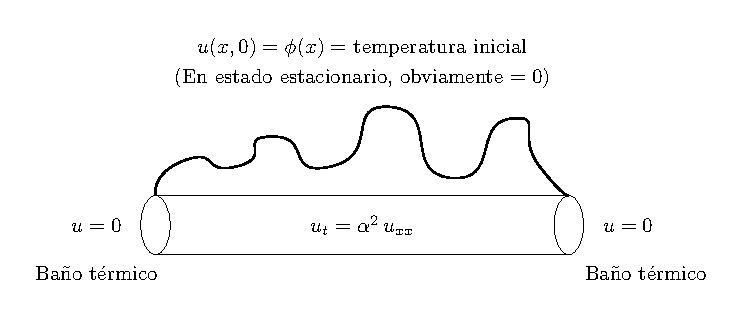
\includegraphics[scale=0.9]{Imagenes/Separacion_Variables_00_Barra.eps}
    \caption{Esquema que representa la barra conductora así como las condiciones iniciales y de frontera.}
    \label{fig:figura_barra_01}
\end{figure}
\end{frame}
\begin{frame}
\frametitle{Revisando previamente el problema}
También se nos dan datos sobre el problema en forma de condición inicial.
\\
\bigskip
\pause
Nuestro objetivo es encontrar la temperatura $u (x, t)$ en valores posteriores al tiempo inicial.
\end{frame}

\subsection{La técnica de separación de variables}

\begin{frame}
\frametitle{Suposición inicial}
El método de separación de variables \emph{supone la existencia de soluciones sencillas} de una EDP de la forma:
\pause
\begin{align*}
u(x, t) =  X(x) \, T(t)
\end{align*}
\pause
donde $X (x)$ es alguna \emph{función que depende solo de} $x$ y $T (t)$ es alguna \emph{función que depende solo de} $t$.
\end{frame}
\begin{frame}
\frametitle{El por qué de las soluciones sencillas}
Las soluciones son sencillas porque cualquier temperatura $u (x, t)$ de esta forma conservará su \enquote{forma} básica para diferentes valores de tiempo $t$, como podemos ver en la figura (\ref{fig:figura_separacion_variables_01})
\end{frame}
\begin{frame}
\frametitle{Esquema de las soluciones sencillas}
\begin{figure}[H]
    \centering
    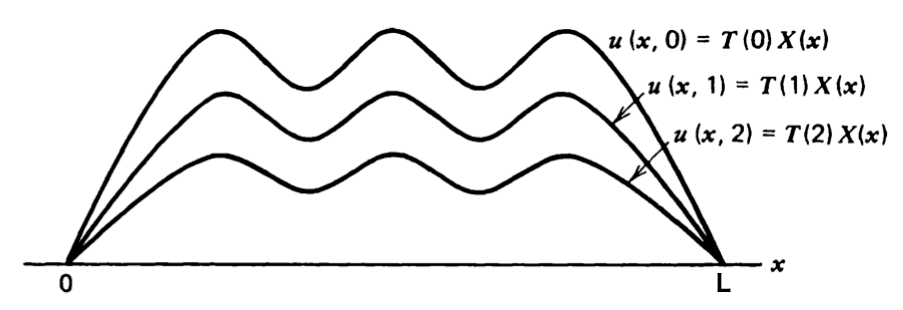
\includegraphics[scale=0.35]{Imagenes/Separacion_Variables_01.png}
    \caption{Gráfica de $X(x)$ y $T(t)$ para distintos valores de $t$.}
    \label{fig:figura_separacion_variables_01}
\end{figure}
\end{frame}
\begin{frame}
\frametitle{Acotando las soluciones}
La idea general que tenemos nos plantea la posibilidad de encontrar un número infinito de estas soluciones a la EDP (que al mismo tiempo también satisfacen las condiciones de frontera).
\end{frame}
\begin{frame}
\frametitle{Las funciones sencillas}
A estas funciones sencillas
\begin{align*}
u_{n} (t) = X_{n} (x) \, T_{n}(t)
\end{align*}
\pause
se les denomina \textbf{soluciones fundamentales}, son las componentes básicas de nuestro problema, y de la solución $u (x, t)$ que estamos buscando.
\end{frame}
\begin{frame}
\frametitle{Sumando soluciones fundamentales}
Sumando las soluciones fundamentales $X_{n}(x) \, T_{n} (t)$ de tal manera que la suma resultante
\pause
\begin{align*}
\sum_{n=1}^{\infty} A_{n} \, X_{n} (x) \, T_{n} (t)
\end{align*}
\pause
satisface las condiciones iniciales. \pause Dado que esta suma aún satisface la EDP y las CDF, ahora tenemos la solución a nuestro problema. Veamos a detalle el método de separación de variables.
\end{frame}

\subsection{Paso 1}

\begin{frame}
\frametitle{Paso 1 - Soluciones elementales}
\textbf{Encontrar las soluciones elementales de la EDP.}
\pause
Nos interesa encontrar la función $u(x, t)$ que satisfaga las siguientes condiciones:
\begin{align*}
\mbox{EDP} \hspace{1.5cm} &u_{t} = \alpha^{2} \, u_{xx} \hspace{1cm} 0 < x < L, \hspace{0.3cm} 0 < t < \infty \\[0.5em] 
\mbox{CDF} \hspace{1.5cm} &\begin{cases}
    u(0, t) = 0 \\
    u(L, t) = 0
    \end{cases}
    \hspace{1cm}
    0 < t < \infty \\[0.5em]
CI \hspace{1.5cm} & u(x, 0) = \phi (x) \hspace{1cm} 0 \leq x \leq L
\end{align*}
\end{frame}
\begin{frame}
\frametitle{Propuesta de solución}
Para comenzar, buscamos soluciones de la forma $u (x, t) = X(x) \, T (t)$ sustituyendo $X (x) \, T (t)$ en la EDP y resolvemos para  $X (x) \, T (t)$.
\\
\bigskip
\pause
Haciendo esta sustitución obtenemos:
\begin{align*}
X(x) \, \ptilde{T} (t) = \alpha^{2} \, \stilde{X} (x) \, T(t)
\end{align*}
\end{frame}
\begin{frame}
\frametitle{Avanzando en el paso}
La parte que hace todo el trabajo es la siguiente: si \emph{dividimos} cada lado de esta ecuación por $\alpha^{2} \, X(x) \, T(t)$, tenemos que:
\pause
\begin{align*}
\dfrac{\ptilde{T} (t)}{\alpha^{2} \, T(t)} = \dfrac{\stilde{X} (x)}{X(x)}
\end{align*}
\end{frame}
\begin{frame}
\frametitle{Variables separables}
Para obtener lo que se conoce como \emph{variables separables}, es decir, la expresión del lado izquierdo de la igualdad depende solo de $t$, mientras que la expresión del lado derecho\footnote{El primado sencillo indica la diferenciación de primer grado con respecto a la variable señalada, mientras que el primado doble, señala la diferenciación de segundo grado con respecto a la variable que se indica.}, depende solo de $x$.
\end{frame}
\begin{frame}
\frametitle{Variables independientes}
Dado que $x$ y $t$ son independientes entre sí, cada lado debe ser una constante fija (digamos $k$),  por tanto podemos escribir:
\pause
\begin{align*}
\dfrac{\ptilde{T}}{\alpha^{2} \, T} = \dfrac{\stilde{X}}{X} = k
\end{align*}
\end{frame}
\begin{frame}
\frametitle{Variables independientes}
De manera equivalente:
\pause
\begin{align*}
\ptilde{T} - k \, \alpha^{2} \, T &= 0 \\[0.5em]
\stilde{X} - k \, X &= 0
\end{align*}
\pause
Entonces, ahora podemos resolver cada uno de estas dos EDO, para luego multiplicarlas y así obtener una solución a la EDP (toma en cuenta que esencialmente hemos cambiado una EDP de segundo orden a dos EDO)
\end{frame}
\begin{frame}
\frametitle{La constante de separación}
Sin embargo, ahora hacemos una observación importante, a saber, queremos que la constante de separación $k$ sea negativa (o de lo contrario el factor $T (t)$ no se anula cuando $t \to \infty$).
\\
\bigskip
\pause
Teniendo esto en cuenta, es una práctica general cambiar el nombre de $k = - \lambda$, donde $\lambda$ es distinta de cero. 
\end{frame}
\begin{frame}
\frametitle{La constante de separación}
Llamando a nuestra \emph{constante de separación} por su nuevo nombre, ahora podemos escribir las dos EDO como:
\begin{align*}
\ptilde{T} + \lambda \, \alpha^{2} \, T &= 0 \\[0.5em]
\stilde{X} + \lambda \, X &= 0
\end{align*}
\pause
Ahora podemos resolver ese par de ecuaciones.
\end{frame}
\begin{frame}
\frametitle{Resolviendo las EDO}
Para $\stilde{X} + \lambda \, X = 0$, las soluciones son de la forma:
\pause
\begin{align}
\begin{cases}
X(x) = A + B \, x & \hspace{0.2cm} \lambda = 0 \\
X(x) = A \, e^{a x} + B \, e^{-a x} & \hspace{0.2cm} \lambda = - a^{2} \\
X(x) = A \cos (a x ) + B \, \sin (a x) & \hspace{0.2cm} \lambda = a^{2}
\end{cases}
\label{eq:ecuacion_06_02_31}
\end{align}
\end{frame}
\begin{frame}
\frametitle{Resolviendo las EDO}
Mientras que para $\ptilde{T} + \lambda \, \alpha^{2} \, T = 0$ se tiene:
\pause
\begin{align}
T(t) = A \, e^{- \lambda \, \alpha^{2} \, t} \hspace{1.5cm} \mbox{con A arbitraria}
\label{eq:ecuacion_06_02_36a}    
\end{align}
y de aquí
\begin{align*}
u(x, t) = X(x) \, T(t) 
\end{align*}
\pause
En este punto, tenemos un número infinito de funciones que satisfacen la EDP.
\end{frame}

\subsection{Paso 2}

\begin{frame}
\frametitle{Paso 2 - Soluciones con las CDF}
\textbf{Encontrar las soluciones de la EDP con las CDF.}
\pause
Ahora debemos de considerar un subconjunto de las soluciones obtenidas en el paso anterior, que a su vez satisfagan las condiciones de frontera (CDF):
\begin{align*}
u(0, t) &= 0 \\[0.5em]
u(L, t) &= 0
\end{align*}
\end{frame}
\begin{frame}
\frametitle{Soluciones con las CDF}
Por las CDF, únicamente en las posibles soluciones para $X(x)$ (ec. \ref{eq:ecuacion_06_02_31}), la tercera posibilidad produce una solución no trivial:
\begin{align*}
X(x) = A \cos (a x ) + B \, \sin (a x), & \hspace{0.2cm} \lambda = a^{2}
\end{align*}
\end{frame}
\begin{frame}
\frametitle{Soluciones con las CDF}
De hecho, trabajando con
\begin{align*}
X(x) = A \cos (a x) + B \, \sin (a x) \hspace{2cm}
\end{align*}
\pause
que al susituir en la solución, multiplicando la solución de $X(t)$ y de $T(t)$:
\begin{eqnarray*}
u(0, t) &=& A \, e^{-\lambda \alpha^{2} \, t} = 0 \pause \hspace{0.3cm} \Longrightarrow \hspace{0.3cm} A = 0 \\[0.5em] \pause
u(L, t) &=& B \, e^{-\lambda \alpha^{2} \, t} \, \sin (\lambda \, L) = 0 \pause \hspace{0.3cm} \Longrightarrow \hspace{0.3cm} \sin (\lambda \, L) = 0
\end{eqnarray*}
\end{frame}
\begin{frame}
\frametitle{Restricción en la constante de separación}
Esta última CDF restringe la constante de separación $\lambda$ de ser cualquier número distinto de cero, debe ser una raíz de la ecuación $\sin (\lambda \, L) = 0$.
\\
\bigskip
\pause
En otras palabras, para que $u(L, t) = 0$, es necesario elegir
\begin{align}
\lambda \, L = n \, \pi \hspace{1.5cm} n \in \mathbb{Z}
\label{eq:ecuacion_06_02_34}    
\end{align}
\end{frame}
\begin{frame}
\frametitle{Conjunto infinito de soluciones}
Sin embargo, para no contar dos veces la misma solución, se toma $n$ positivo, es decir:
\begin{align}
\lambda = \dfrac{n^{2} \, \pi^{2}}{L^{2}} \hspace{1.5cm} n = 1, 2, 3, \ldots
\label{eq:ecuacion_06_02_35}
\end{align}
\pause
En este paso hemos encontrado un número infinito de funciones que son solución a la EDP:
\begin{align}
u_{n} (x, t) = A_{n} \, \exp \left( - \dfrac{n^{2} \, \alpha^{2} \, \pi^{2}}{L^{2}} \, t \right) \, \sin \left( \dfrac{n \, \pi}{L} \, x \right)
\label{eq:ecuacion_06_02_37}    
\end{align}
\end{frame}
\begin{frame}
\frametitle{Usando el principio de superposición}
Por el principio de superposición, la solución que se propone es:
\pause
\begin{align}
u (x, t) = \sum_{n=1}^{\infty} A_{n} \, \exp \left( - \dfrac{n^{2} \, \alpha^{2} \, \pi^{2}}{L^{2}} \, t \right) \, \sin \left( \dfrac{n \, \pi}{L} \, x \right)
\label{eq:ecuacion_06_02_38}
\end{align}
\pause
Nos queda por considerar las condiciones iniciales del problema para obtener entonces la solución a la EDP.
\end{frame}

\subsection{Paso 3}

\begin{frame}
\frametitle{Paso 3 - Solución con la CI}
\textbf{Encontrar la solución de la EDP, con las CDF y la condición inicial.}
\\
\bigskip
\pause
El último paso (y probablemente el más interesante desde un punto de vista matemático) es agregar las soluciones fundamentales (ec. \ref{eq:ecuacion_06_02_38}) de tal manera (eligiendo los coeficientes $A_{n}$) que la condición inicial:
\pause
\begin{align*}
u(x, 0) = \phi (x)
\end{align*}
se satisfaga.
\end{frame}
\begin{frame}
\frametitle{Usando la CI}
Utilizando la CI en la suma, se tiene que:
\begin{align*}
\phi (x) = \sum_{n=1}^{\infty} A_{n} \, \sin \left( \dfrac{n \, \pi}{L} \, x \right)
\end{align*}
\pause
Vemos que esto es equivalente a encontrar el desarrollo en series de la función seno de $\phi (x)$.
\end{frame}
\begin{frame}
\frametitle{Solución en series}
Se debe de ocupar el desarrollo en una serie de Fourier y ocupar la propiedad de ortogonalidad de la función seno.
\\
\bigskip
\pause
Por lo que:
\begin{align}
A_{n} = \dfrac{2}{L} \int_{0}^{L} \phi (x) \, \sin \left( \dfrac{n \, \pi}{L} \, x \right) \dd{x}
\label{eq:ecuacion_06_02_40}    
\end{align}
\end{frame}
\begin{frame}
\frametitle{Solución completa al problema}
Entonces la solución completa al problema de Dirichlet para la ecuación de calor es:
\begin{align*}
u (x, t) &= \dfrac{2}{L} \sum_{n=1}^{\infty} \left[ \int_{0}^{L} \phi (x) \, \sin \left( \dfrac{n \, \pi}{L} \, x \right) \dd{x} \right] \times \\[1em]
&\times \exp \left( - \dfrac{n^{2} \, \alpha^{2} \, \pi^{2}}{L^{2}} \, t \right) \, \sin \left( \dfrac{n \, \pi}{L} \, x \right)
\end{align*}
\end{frame}
\end{document}